\section{Objectifs :}

Formulation du besoin sous forme de bête à cornes :
\begin{figure}[h]
	\begin{center}
		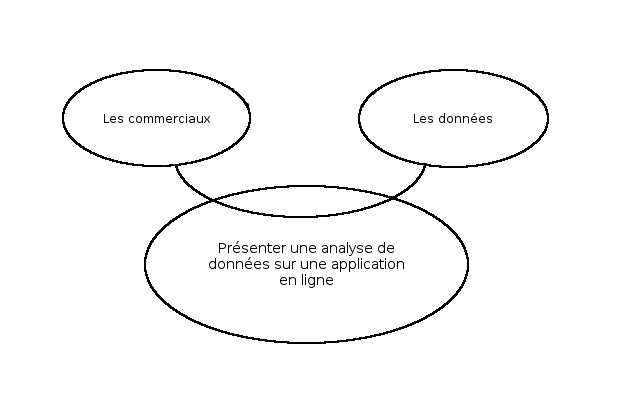
\includegraphics[scale=0.5]{img/beteCornes.png}
		\caption{Bête à cornes}
	\end{center}
\end{figure}

En partant du cahier des charges nous avons réalisé une première liste des fonctionnalités à implémenter sur notre application :

\paragraph{Partie utilisateur :}
\begin{enumerate}
\item[•] Page d'accès au site : doit comprendre une page de connexion avec un mail et un mot de passe, ainsi qu'une option pour faire une demande d'accès auprès de l'administrateurs.
\item[•] Tableau de bord : page principale du site. L'utilisateur doit être redirigé vers cette page après la connexion. Cette page doit contenir tous les graphiques et statistiques nécessaires à l'utilisateur. C'est ici que l'utilisateur doit pouvoir trouver toutes les informations que nous avons extraites de la base de données. De plus, il y aura sur cette page un lien vers la page de géolocalisation.
\item[•] Page de Géolocalisation : sur cette page l'utilisateur devra pouvoir observer comment se répartissent dans l'espace les données fournies par le tableau de bord. Elle contiendra donc une carte Google Map et affichera des zones de couleurs en fonction de critères choisis par l'utilisateur (chiffre d'affaires, marges, ...).
\item[•] Page d'aide : contient tout simplement le manuel d'utilisation de l'application.
\end{enumerate}

\paragraph{Partie administrateur :} La partie administrateur permettra de gérer l'ensemble du site. Les données ainsi que les utilisateurs doivent être validés par l'administrateur. Nous appelerons cette partie de notre site le Back-office. Celui devra permettre :
\begin{enumerate}
\item[•] Le téléchargement de fichiers pour alimenter la base de données.
\item[•] La gestion des comptes utilisateurs.
\end{enumerate}